%versi 2 (8-10-2016) 
\chapter{Pendahuluan}
\label{chap:intro}
   
\section{Latar Belakang}
\label{sec:label}
Ujian menjadi salah satu syarat yang mutlak untuk memenuhi komponen penilaian
suatu mata kuliah. Salah satu bentuk ujian tersebut dilakukan secara praktik.
Ujian praktik ini dilaksanakan pada lab komputasi dengan bantuan aplikasi. Pihak
yang bertanggung jawab untuk mempersiapkan ruangan dan sistem adalah
\textit{System Administrator} atau Admin. Peserta akan diberi soal ujian melalui
sistem yang berjalan di lab sesuai prosedur dan aturan yang berlaku.

Ujian pada Lab Komputasi dilakukan dengan bantuan aplikasi. Aplikasi tersebut
membantu mengatur berbagai kebutuhan seperti pengumpulan jawaban, pengacakan
daftar peserta, serta pengarsipan berkas jawaban. Aplikasi yang saat ini
digunakan bernama Oxam (Gambar \ref{fig:ss-Oxam}). Oxam bekerja dengan meminta
parameter berupa kode matakuliah, tipe ujian, jurusan, jam mulai ujian, daftar
peserta, \textit{slot} tempat duduk yang dapat digunakan, dan daftar nama berkas
yang akan dikumpulkan. Aplikasi Oxam akan secara otomatis membuatkan daftar
tempat duduk peserta yang sudah teracak, dan membuatkan \textit{script} untuk
menyalin berkas ujian ke komputer peserta.

\begin{figure}
    \centering
    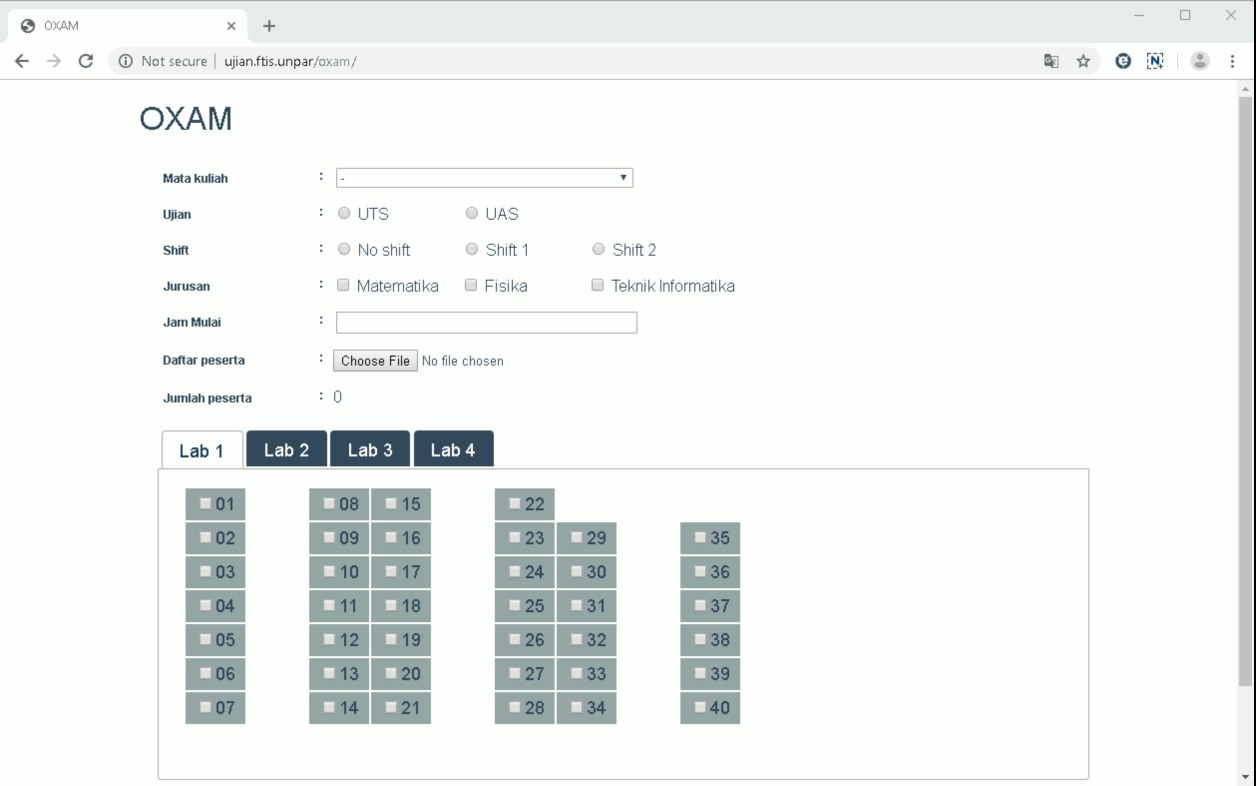
\includegraphics[width=0.7\paperwidth]{Gambar/ss-oxam.png}
    \caption{Tampilan cuplikan layar dari Oxam, aplikasi manajemen ujian di Lab Komputasi.}
    \label{fig:ss-Oxam}
\end{figure}

Namun fitur yang terbatas membuat Oxam menjadi tidak efektif untuk menyelesaikan
insiden-insiden khusus. Salah satu masalah yang sering dihadapi adalah
pemindahan posisi peserta ke meja lain saat masalah terjadi. Admin harus
mengubah secara manual entri pada basis data yang bersangkutan, lalu memindahkan
berkas ujian tersebut secara manual ke posisi yang baru. Selain itu dengan
berubahnya NPM (Nomor Pokok Mahasiswa) untuk angkatan 2018 dan selanjutnya
membuat sistem Oxam yang lama tidak dapat digunakan tanpa harus mengubah NPM
tersebut ke bentuk yang lama. Perubahan tersebut dapat dilihat pada Tabel
\ref{tab:table-npm}. 

\begin{table}[H]
    \centering
    \def\arraystretch{2}
    \begin{tabular}{|c|c|}
        \hline
        \textbf{NPM Lama} & \textbf{NPM Baru} \\
        \hline
        201673\textbf{0011} & 6181601\textbf{011} \\
        \hline
    \end{tabular}
    \caption{NPM lama dan NPM baru yang sistem informasi gunakan.}
    \label{tab:table-npm}
\end{table}

Karena sistem Oxam tertegrasi dengan layanan server lain, maka NPM harus
distandarisasi dengan memetakan NPM ke username. Pemetaan NPM menjadi username
ini menjadi bermasalah karena perbedaan struktur NPM yang berbeda. Perbedaan ini
meliputi seperti, nomor kode jurusan (Informatika adalah 73, saat ini menjadi
618), lalu posisi tahun yang berpindah dan adanya kode reguler (01) dan
non-reguler pada depan nomor urut. Perbedaan ini membuat sistem lama tidak dapat
memetakan NPM baru ke username yang biasanya digunakan oleh sistem yang sudah
ada di lab komputasi saat ini.

Selain itu runtutan kegiatan yang dilakukan pada saat fase persiapan ujian pada
Lab Komputasi dengan aplikasi ini terlalu banyak. Berdasarkan pengalaman,
hal ini menimbulkan beberapa \textit{human error} sebagai berikut:
    \begin{itemize}
        \item Berkas daftar duduk peserta yang tertimpa oleh sesi ujian
            berikutnya. Berkas daftar tempat duduk dibuat menjadi berkas HTML
            yang harus dicetak. Daftar berkas tersebut dapat dilihat pada Gambar
            \ref{fig:ss-folder-gen}.\\
            Jika Admin lupa mencetak atau menyalin berkas tersebut ke komputer
            lokal, Admin tersebut diharuskan untuk menghapus entri ujian
            tersebut, lalu mendaftarkan ulang sesi ujian tersebut beserta dengan
            daftar peserta dan daftar tempat duduk yang digunakan.

        \item Jika Admin melakukan \textit{copy} dengan urutan yang salah, \textit{folder} untuk
            ujian tidak akan terbuat, atau bahkan tidak dapat diakses oleh peserta.
        
        \item Salah memasukkan daftar peserta ujian.
        
        \item Menghapus folder berkas ujian yang lama pada server. Jika petugas
            tersebut lupa, maka konsekuensinya adalah pada saat pengumpulan,
            Admin yang bertugas harus memisahkan berkas ujian lama dan yang baru
            secara manual.
    \end{itemize}

\begin{figure}
    \centering
    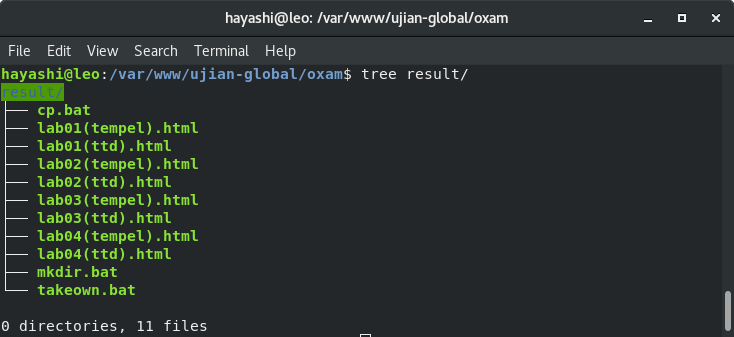
\includegraphics[width=0.7\paperwidth]{Gambar/ss-struktur-folder-generator.png}
    \caption{Daftar peserta yang di\textit{generate} oleh Oxam dalam bentuk
    berkas.}
    \label{fig:ss-folder-gen}
\end{figure}

Masalah berikutnya muncul pada saat proses ujian tersebut berjalan. Pertama,
terdapat \textit{bug} waktu ujian telah habis, pada kenyataannya waktu ujian
belum habis. Kedua, \textit{timer} yang digunakan untuk menunjukan sisa waktu
ujian tidak tersingkronisasi dengan Oxam. Sehingga pada saat timer berbunyi,
tempat pengumpulan tidak langsung tertutup. Ketiga, entri ujian yang sudah
dihapus masih muncul pada tempat pengumpulan. Hal ini biasanya diatasi oleh tim
admin dengan cara mengubah tanggal sesinya ke tahun lalu.

Pada fase pengumpulan berkas jawaban ujian ke dosen koordinator, sistem tidak
secara otomatis mengumpulkan berkas tersebut. Sehingga seringkali Admin yang
bertugas lupa untuk mengirimkan berkas tersebut. Pengumpulan berkas tersebut
seharusnya dikirimkan sesegera mungkin saat ujian sudah selesai. Hal ini
dimaksudkan agar jawaban tidak diubah di kemudian hari tanpa izin.

Selain masalah-masalah pada tiap fase tersebut, masalah lain ada pada sistem itu
sendiri. Oxam menyimpan berkas tanpa mengacak lokasi atau nama berkas jawaban
tersebut, diperlihatkan pada Gambar \ref{fig:ss-folder-jawaban}. Hal ini dapat
mempermudah penyerang sistem untuk mengubah berkas jawaban tersebut.

\begin{figure}
    \centering
    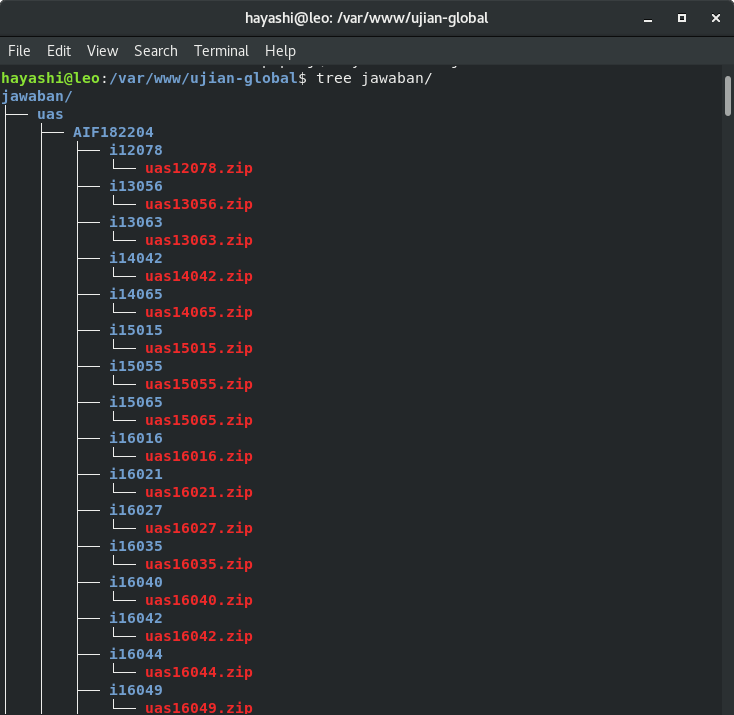
\includegraphics[width=0.6\paperwidth]{Gambar/ss-struktur-folder-jawaban.png}
    \caption{Struktur folder jawaban pada sistem Oxam.}
    \label{fig:ss-folder-jawaban}
\end{figure}

Pada penelitian ini, akan dibangun ulang aplikasi baru untuk
menyelesaikan masalah-masalah yang muncul pada aplikasi lama dengan
menggunakan \textit{framework Fat-free} dan \textit{React}.

\section{Rumusan Masalah}
\label{sec:rumusan}
Pada skripsi ini, aplikasi akan membantu memecahkan masalah:
\begin{itemize}
    \item Apa saja kebutuhan aplikasi untuk ujian untuk sistem manajemen
    ujian di lab komputasi?
    
    \item Bagaimana implementasi pemenuhan kebutuhan aplikasi sistem
    manajemen ujian di lab komputasi?
\end{itemize}

\section{Tujuan}
\label{sec:tujuan}
Tujuan dari skripsi ini adalah sebagai berikut:
\begin{itemize}
    \item Melakukan survei dan analisis untuk mendapatkan daftar kebutuhan
        aplikasi ujian untuk aplikasi pendukung manajemen ujian di lab
        komputasi.

    \item Pemenuhan kebutuhan diimplementasi dengan membuat ulang perangkat
        lunak dengan menggunakan \textit{framework}, dengan harapan dapat terus
        dipelihara oleh tim admin di kemudian hari.

\end{itemize}

\section{Batasan Masalah}
\label{sec:batasan}
Batasan masalah pada penelitian ini adalah sebagai berikut:
\begin{enumerate}
    \item Aplikasi pendukung ujian akan berjalan pada server berbasis Linux,
        sehingga dibutuhkannya bantuan untuk mengeksekusi \textit{script batch}
        pada sistem operasi Windows.
        
    \item \textit{Script} yang dihasilkan hanya mendukung untuk sistem operasi Windows.
\end{enumerate}

\section{Metodologi}
Metodologi yang dilakukan pada penelitian ini adalah sebagai berikut:
\label{sec:metlit}
    \begin{enumerate}
        \item Studi literatur bahasa dan \textit{framework} Fat-free dan
            \textit{libary} React.js.
        \item Melakukan survei sistem dan menyebar kuisioner mengenai sistem ujian 
            yang berjalan pada lab.
		\item Melakukan perancangan ERD basis data aplikasi Oxam.
		\item Melakukan perancangan tampilan antarmuka aplikasi Oxam.
		\item Mengimplementasi modul/entitas berikut:
		    \begin{itemize}
		        \item Mata Kuliah
		        \item Peserta Ujian
		        \item Ujian (Sesi Ujian)
		        \item Print Daftar Peserta
		        \item Pengumuman untuk Peserta
		    \end{itemize}
	     \item Implementasi Tampilan untuk Peserta dengan detil:
		    \begin{itemize}
		        \item Tempat Pengumpulan
		        \item \textit{Sumary} Ujian
		        \item Bagian informasi/notifikasi
		    \end{itemize}
		\item Implementasi Admin Panel untuk Admin.
	    \item Melakukan \textit{deployment} dan pengujian pada fungsionalitas
	        aplikasi.
	    \item Implementasi pengiriman berkas jawaban ujian secara otomatis ke
	        dosen bersangkutan.
        \item Menarik kesimpulan dan saran berdasarkan proses penelitian dan
            pengujian.
    \end{enumerate}

\section{Sistematika Pembahasan}
\label{sec:sispem}

Pembahasan penelitian akan dilakukan secara sistematis dengan detail sebagai
berikut:

\begin{itemize}
    \item Bab 1 Pendahuluan \\
        Berisi latar belakang dibuatnya penelitian aplikasi manajemen ujian di lab komputasi, 
        rumusan masalah, tujuan, batasan masalah, metodologi serta sistematika pembahasan penelitian ini.
    
    \item Bab 2 Landasan Teori \\
        Bab ini berisi Pedoman Pelaksanaan Ujian di Lab Komputasi, landasan
        teori dari Aplikasi Berbasis Web, \textit{Framework} dan
        \textit{Library}, REST API, CI/CD serta Docker yang akan menjadi
        landasaan untuk membantu analisis penelitian aplikasi manajemen ujian di
        lab komputasi.
        
    \item Bab 3 Analisis \\
        Berisi pembahasan analisa sistem ujian masa kini pada lab komputasi,
        pelaksanaan ujian, analisa kebutuhan dan fitur aplikasi Oxam berdasarkan
        kuisioner, pemilihan \textit{framework} dan \textit{library}, serta
        Analisis pengguna.
        % TODO scenario
        
    \item Bab 4 Perancangan \\
        Pada bab ini akan dijabarkan tentang perancangan aplikasi yang akan
        diimplementasi untuk membantu memanajemen ujian di lab komputasi.
        Perancangan tersebut akan terdiri dari perancangan tampilan antar muka
        untuk peserta, admin, layar proyektor dan lembar jawab. Lalu perancangan
        dilakukan juga untuk basis data, API, juga sistem CI/CD.
    
    \item Bab 5 Implementasi dan Pengujian \\
        Berisi pembahasan implementasi aplikasi yang telah dirancang dan
        pengujian aplikasi tersebut. Pengujian akan terdiri dari pengujian
        eksperimental dan fungsional.
        
    \item Bab 6 Kesimpulan dan Saran \\
        Berisi kesimpulan dan saran dari penelitian aplikasi manajemen ujian di
        lab komputasi berdasarkan perancangan, implementasi dan pengujian yang
        telah dilakukan.
\end{itemize}